\documentclass[11pt]{p9article}
\usepackage{graphicx}
\usepackage{epsfig}
%\usepackage{subfigure}
\usepackage{subfig}

\textwidth 150mm
\textheight 220mm
\topmargin +5mm
\oddsidemargin 0mm
\evensidemargin 0mm
\setlength\parindent{0pt}
\setlength\parskip{0.25\baselineskip}
\renewcommand\baselinestretch{0.8}
\renewcommand{\familydefault}{\sfdefault}

\makeatletter
\renewcommand\section{\@startsection {section}{1}{\z@} {3pt} {1pt} {\normalfont\normalsize\bfseries}}
\renewcommand\subsection{\@startsection {subsection}{1}{\z@} {3pt} {1pt} {\normalfont\normalsize\bfseries}}
\makeatother

\begin{document}
\title{\Large\textbf{Gostor: Storage beyond POSIX}}
\author{\large 
	\begin{tabular}{c}
	\textsl{Latchesar Ionkov}\\
	\textsl{Los Alamos National Laboratory\footnote{LANL publication: LA-UR-11-11422}}\\
	\texttt{lionkov@lanl.gov}\\\\
	\end{tabular}
}

\maketitle\thispagestyle{empty}
\pagestyle{empty}

\begin{abstract}

\setlength\parindent{0pt}
\setlength\parskip{0.25\baselineskip}
	Gostor is an experimental platform for testing new file
	storage ideas for post POSIX usage. Gostor provides greater
	flexibility for manipulating the data within the file,
	including inserting and deleting data anywhere in the file,
	creating and removing holes in the data, etc. Each
	modification of the data creates a new file. Gostor doesn't
	implement any ways of organizing the files in hierarchical
	structures, or mapping them to strings. Thus Gostor can be
	used to implement standard file systems as well as
	experimenting with new ways of storing and accessing users'
	data.
\end{abstract}


\section{Introduction}

Currently there are two popular ways of storing data -- hierarchical
file systems, and relational databases. The hierarchical file systems
consist of {\bfseries files} (arrays of bytes) that have names. The
files are grouped in {\bfseries directories} which can be members of
other directories. In order to access a file, one needs to know the
{\bfseries path}, i.e. the list of directories from {\bfseries root}
of the file system. Files data can be overwritten, but new data can be
added only at the end of the file. Most of the popular file systems
support the POSIX (or similar) set of file
operations~\cite{IEEE:POSIX.1-90}. Relational databases enforce strong
structure on the stored data, by enforcing it to be fitted in a set of
tables. The data can be accessed by using the SQL language. Relational
databases provide better consistency and concurrency guarantees. They
are hard to install and maintain, often requiring professional
database administrator in order to achieve reasonable performance.

There are many attempts to introduce some of the database benefits to
the file systems, such as transactions, snapshots, etc. Even though
some of the popular file systems support snapshots and versioning,
creating and manipulating snapshots is not part of the standard file
operations.

In many cases, especially with scientific datasets, extending files
only at the end is too restrictive. To avoid the limits, some
scientific data formats, like HDF~\cite{hdf} re-implement most of the
file system data structures in the file.

There are some attempts to go beyond both hierarchical naming of files
as well as relaxation on the restrictions on how the content of the
files can be modified.
hFAD~\cite{Seltzer:2009:HFS:1855568.1855569} allows data to be
inserted and deleted at any place in the file. It also removes the
dependency on file names when accessing the files and allows adding
tags that describe the content of the files. 

Most of the attempts to change the way data is stored and accessed are
built on top of standard file systems or databases.

Gostor is a low-level storage system that provides consistent way of
manipulating arrays of bytes, providing both versioning support as
well as ability to insert, delete and modify data anywhere within the
array. It also allows insertion and removal of holes in the array.

Gostor avoids the issues with hierarchical file names by not
supporting them. All files in Gostor are immutable and can be accessed
by a 64-bit ID that is returned when they are created. Files are
created by cloning already existing files and modifying some of file's
data.

\section{Gostor Architecture}


\subsection{Files}

A {\bfseries file} in Gostor is an immutable string of bytes. Regions
of file where data haven't been written are holes in the file. They
are not stored and don't use disk space. Reading from a hole region
returns zeroes.

A file is identified with a 64-bit integer called {\bfseries fileID}.
The fileID may change during the life span of the file. If the
fileID is changed, Gostor guarantees that all references to the old
fileID within the storage will be modified, and that the old fileID
can be used until they are specifically discarded, or the connection
to Gostor is closed. There is no guarantee that a fileID retrieved
during previous connection will still be valid when a new connection
is established.

File with fileID 0 always points to a zero-length file.

\subsection{Data Content Types}

When reorganizing the disk space, Gostor needs to know if any of the
files contain references to other files. For that reason all data
stored is assigned {\bfseries data content type}. When writing data to
files, the user can specify whether the data contains references to
other files. Because data type is specified by write, there is no
restriction for the whole file to have the same data content type.
Gostor can coalesce content of data written by multiple writes as long
as it is sequential and of the same type. When data is read, Gostor
returns only data of the same content type.

Currently there are only two data types available to the user:

\begin{tabular}{lp{9cm}}
Data Type & Description \\
\hline
{\bfseries BTData} & Data that doesn't contain any fileIDs \\
{\bfseries BTDir} & File content with only fileIDs \\
\end{tabular}

Gostor defines additional data content types that are used internally
to implement the file layout.

Gostor allows up to 32 thousand data types defined, but currently
doesn't provide operations in the protocol for creating new data
types. Extensions to Gostor (such as file systems) can use an internal
API.

\subsection{Operations}

\subsubsection{Read}

\begin{verbatim}
    read(file, offset uint64, buf []byte) (count int, dtype uint16,
        err os.Error)
\end{verbatim}

The {\bfseries read} function reads up to length of the \verb|buf|
array bytes from the specified file, starting from the specified
\verb|offset| and stores it in the \verb|buf| array. It returns the
number of bytes returned as well as the data content type of the data.
If an error occurs while reading, \verb|err| contains the error.

Read can return less than \verb|len(buf)| bytes in two cases -- if there is no
more data in the file (i.e. \verb|offset + len(buf)| is greater than the
file's size), or if the data in the file has mixed data content types.

\subsubsection{Write}

\begin{verbatim}
    write(file, soffset, eoffset uint64, count uint32, data []byte,
        dtype uint16) (newfile uint64, err os.Error)
\end{verbatim}

Because Gostor files are immutable, each write operation creates a new
file. It receives an existing file as argument, clones its content,
applies the changes of the data content and returns the fileID of the
newly created file.

The write call is used to do any modifications to a file. It replaces
the data currently located between offsets \verb|(soffset, eoffset)|
with \verb|count| bytes containing the data from the \verb|data|
array. If the length of the \verb|data| array is less than
\verb|count|, a hole is created at the end of the region. Table
\ref{tab:write} shows examples on how the {\bfseries write} operation
can be used to modify the data.

\begin{table*}[ht]
\begin{center}
\begin{tabular}{lp{8cm}}
Operation & Description \\
\hline
\verb|write(.., 10, 10, 100, data)| & Insert 100 bytes of
		data at offset 10 \\
\verb|write(.., 10, 10, 100, nil)| & Insert 100 byte hole at
		offset 10 \\
\verb|write(.., 10, 110, 0, nil)| & Delete 100 bytes of data
		starting at offset 10 \\
\verb|write(.., 10, 110, 100, data)| & Overwrite 100 bytes of data
		starting at offset 10 \\
\end{tabular}
\caption{Examples on data modifications using {\bfseries write}}
\label{tab:write}
\end{center}
\end{table*}

\subsubsection{Size}
 
\begin{verbatim}
    size(file uint64) (size uint64, err os.Error)
\end{verbatim}

Returns the size of the specified file.

\subsubsection{Forget}

\begin{verbatim}
    forget(file uint64)
\end{verbatim}

Informs Gostor that the user is no longer going to use the file with
the specified fileID. If there are no more references to the file, it
may be garbage-collected.

\section{Current Implementation}

Gostor is implemented in Go. Currently it is approximately 2000 lines
of code.

\subsection{Segments and Blocks}

Gostor uses log-structured data layout, similar to the ones used in
log-structures file systems~\cite{Rosenblum:1991:DIL:121133.121137}.
The disk space is divided into segments, and the segments are kept in
a doubly-linked list. The segments can be {\bfseries free}, {\bfseries
full}, or {\bfseries active}. There is only one active segment at a
time. All new data is appended at the end of the active segment. Once
the segment is full, it is marked as ``full'' and the next segment in
the list is set as active.

The space within the segments is not divided into fixed-size chunks.
Each segment consists of a number of variable-sized blocks. Each block
can be up to $2^16$ bytes long (including the header). The header of
the block contains its size as well as the type of the data it
contains (data content type). The blocks always start at an even
offset.

Figure~\ref{fig:disk-layout} shows the physical layout of the segments
and the blocks.

\begin{figure*}[ht!]
\begin{center}
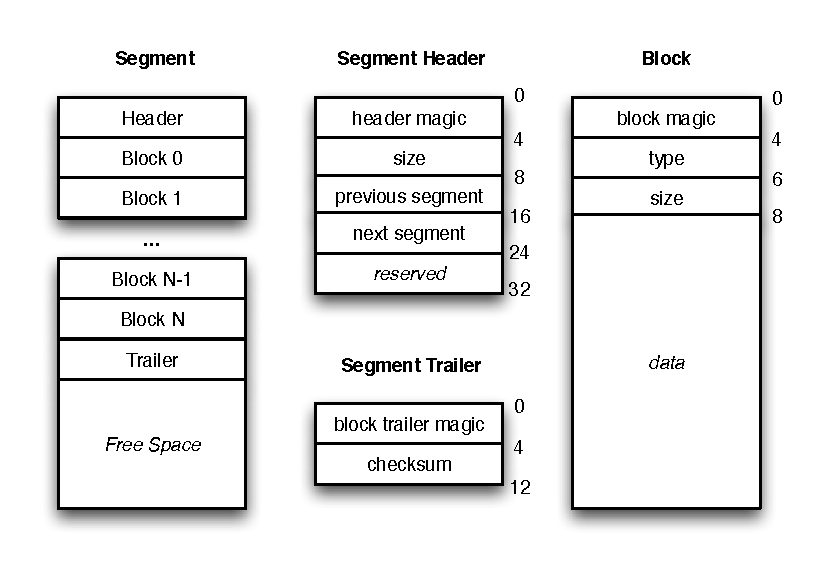
\includegraphics
	[width=0.9\textwidth,keepaspectratio] 
	{disk-layout.eps}
\caption{Gostor Disk Layout}
\label{fig:disk-layout}
\end{center}
\end{figure*}

\subsection{Files}

Gostor uses modification of Btrees to describe files. Blocks at level
0 contain the data of the file. Blocks at level 1 contain entries to
the data blocks at level 0, and so forth. Because Gostor allows
insertion of data anywhere in a file, offsets to data are not constant
and can't be stored in the intermediate Btree blocks. Instead, each
Btree entry contains the size of the data it describes. Normally the
Btree blocks are fixed size and waste some space when there are not
enough entries. Because of the log-structured layout used by Gostor,
the Btree representation we use is compact and doesn't waste any disk
space.

The fileID of a file is the offset (relative to the beginning of the
disk) of the block describing the root of the file Btree. This
approach simplifies the implementation of Gostor and avoids a level of
indirection, that is common to inode based systems.

Figure~\ref{fig:btree} shows an example of a file with fileID 348. The
file's Btree has tree levels. The first entry in the root block points
to block 388 and defines that that block describes the first 1100
bytes of the file. Block 388 has two entries, one is 700 bytes long
and the data is stored in block 500. The second entry describes
400-byte long hole (the block is 0). Figure~\ref{fig:btree} also shows
how the file blocks are laid out in a segment.

\begin{figure*}[ht!]
\begin{center}
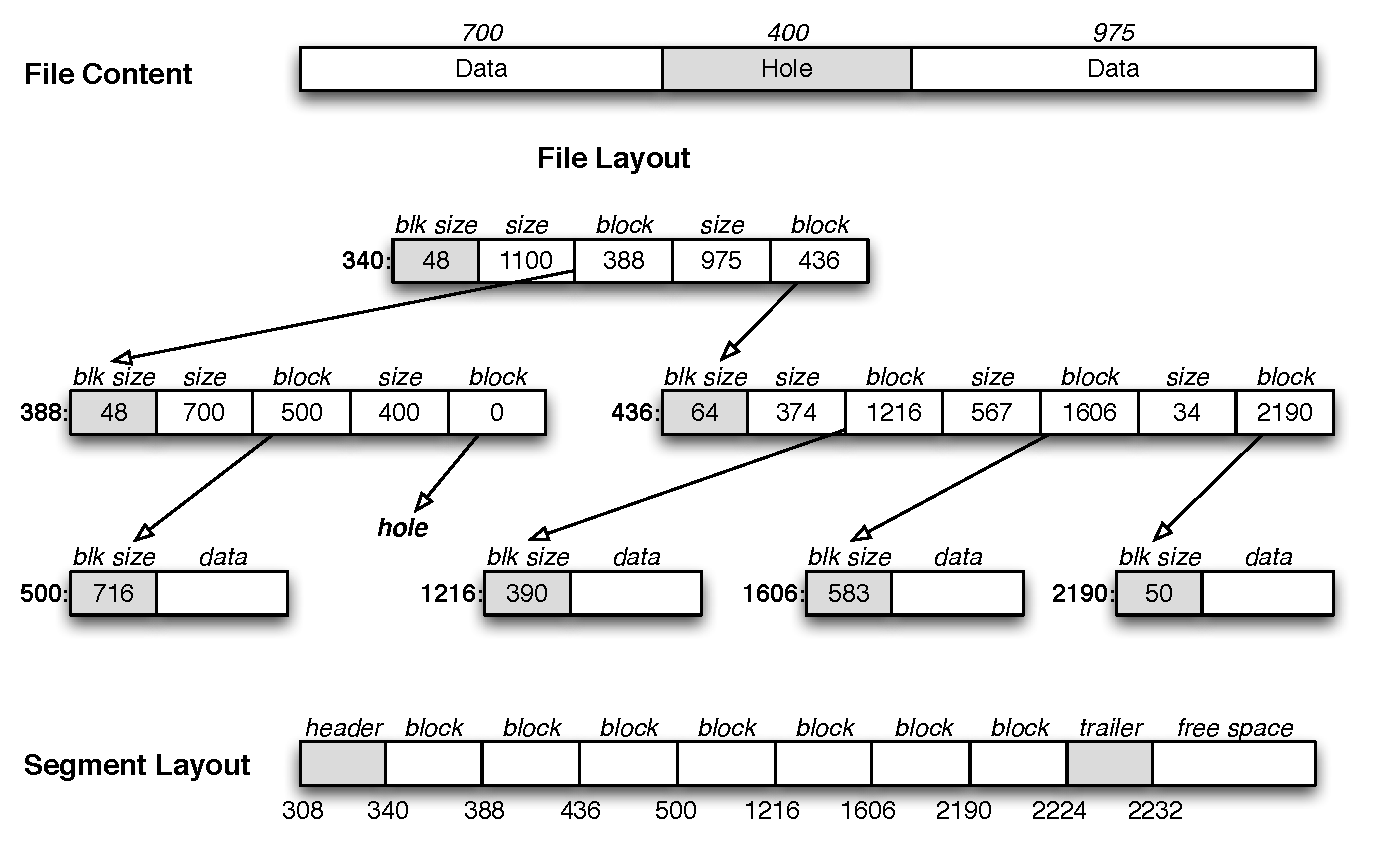
\includegraphics
	[width=0.9\textwidth,keepaspectratio] 
	{btree.eps}
\caption{Btree and Segment Representation of a File}
\label{fig:btree}
\end{center}
\end{figure*}

\subsection{Operations}

The {\bfseries write} operation uses the specified file's Btree as a base for the
Btree of the newly created file. It creates new blocks for a sub-tree
of the file, up to the new file's root block. While building a new
tree, Gostor tries to coalesce neighboring blocks if their size is
less than the allowed size ($2^16$ bytes for level 0 blocks and $8192$
bytes for intermediate blocks). Gostor fills up the intermediate
blocks with entries left-to-right so the rightmost affected block on
the level is left unfilled. This approach is optimized for the
most-frequently use case when data is appended at the end of the file.

Figure~\ref{fig:btree-write} shows the layout of the data when
operation \verb|write(340, 700, 700, 162, data)| is performed on the
file shown on Figure~\ref{fig:btree}. The operation inserts 150 bytes
of data at offset 700 and increases the size of the hole with 12 bytes.

\begin{figure*}[ht!]
\begin{center}
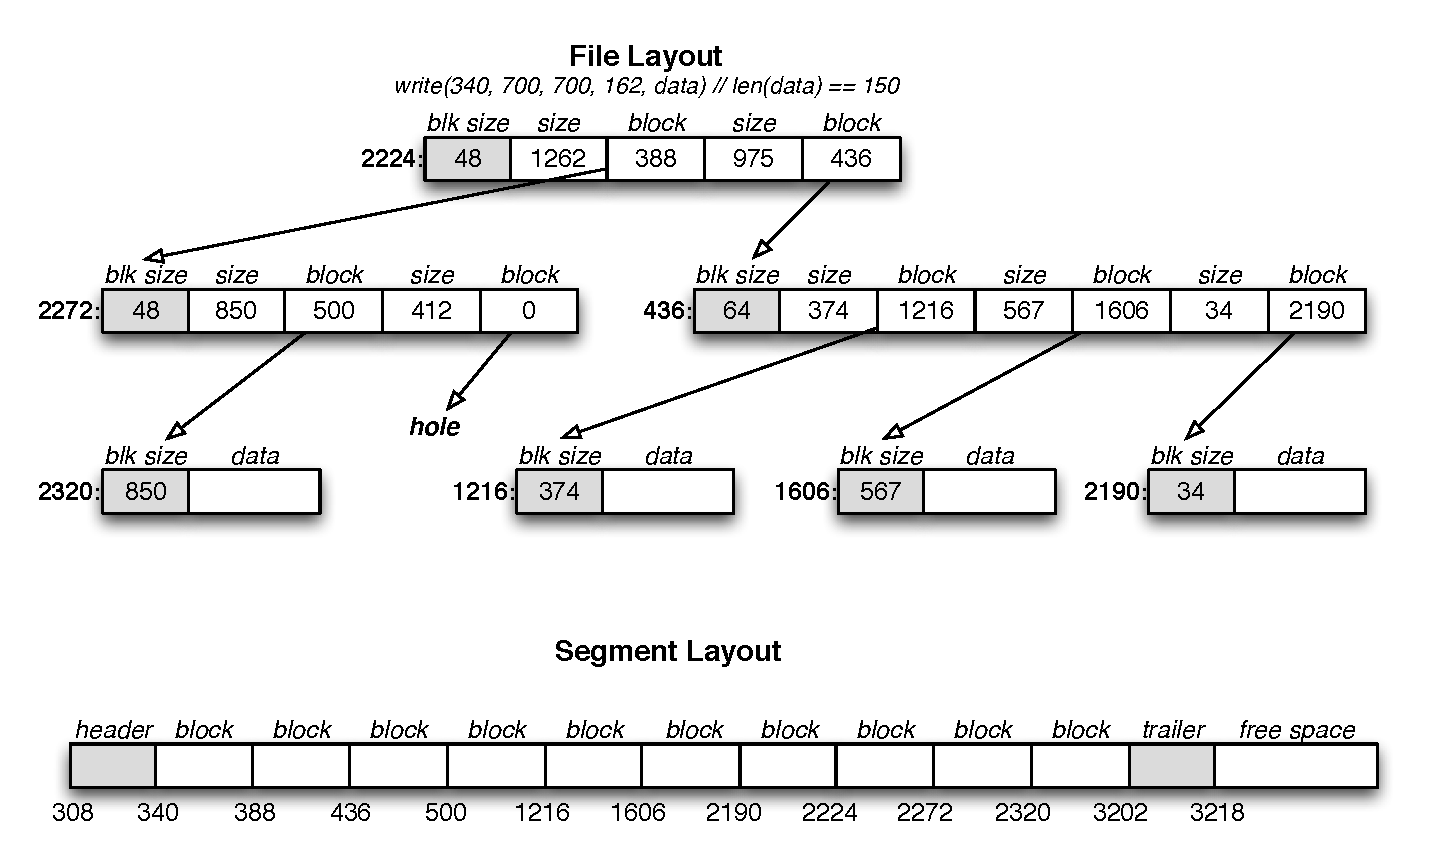
\includegraphics
	[width=0.9\textwidth,keepaspectratio] 
	{btree-write.eps}
\caption{Btree and Segment Representation of a file after {\bfseries write}
operation}
\label{fig:btree-write}
\end{center}
\end{figure*}

\subsection{Garbage Collection}

Each {\bfseries write} operation in Gostor creates a new file with a new root
block, some intermediate Btree blocks as well as some data blocks. In
most cases, once the new file is created, the old file is no longer
useful and the blocks that belong only to it should be recycled.
Gostor has knowledge of all references to blocks stored in it. It
also keeps track of the blocks that the user is using at the moment.
{\bfseries Forget} operation should be called if the user no longer
cares about a block.

Having information which blocks are still in use allows Gostor to
reclaim the space that is no longer accessible. Currently Gostor
supports only in-memory garbage collection. When a block is stored in
Gostor, it is added to an in-memory list of data to be written to the
disk. The data is kept in the memory for some time, giving it a chance
to get obsoleted by subsequent changes to the list of live files. 

When the user is no longer going to use a reference to a block, the
{\bfseries forget} command should be used to update Gostor's knowledge
of what data is regarded as live by the user.

Currently Gostor supports only in-memory garbage collection. Once the
data is committed to the disk, it can't be removed. Writing a garbage
collector for the on-disk data is planned as future work.

\subsection{Committing Blocks to Disk}

When a block is stored in Gostor, it is not written to the disk right
away. In most cases, the data in the block will be obsoleted soon by
subsequent call and premature write to the disk would be wasteful.
Gostor keeps the blocks in memory for some time to allow the data to
be made obsolete. Gostore doesn't have knowledge what blocks will be
actually stored on disk and therefore can't assign disk offsets for
the blocks before they are actually committed. Instead, Gostor returns
temporary offsets that can be used to access the data, or store
references to the block in Gostor.

Before committing the data on disk, Gostor runs the garbage collector
to free all blocks that are no longer live. Then it assigns disk
offsets to the remaining blocks, and updates the temporary offsets
stored in the blocks to the permanent ones. It can do that because it
has knowledge if a block contains references to other blocks. Once the
references are updated, the blocks are stored on the disk. The
temporary offsets can be used until they are ``forgotten''.

\section{Future Work}

The current Gostor implementation doesn't have garbage collector that
can reclaim data already written to the disk. There are plans for
implementing copying, generational garbage collector that crawls
through the existing data and copies the reachable blocks into new
segments. Because of the high penalty of reading all existing data,
the future implementation might be modified so in segregates blocks
that contain references to other blocks in separate segments.

Once the Gostor prototype is stable enough, we plan to implement
conventional hierarchical file system on top of it, as well as
experiment with porting existing formats (HDF5) for scientific data on
top of it.

\bibliography{gostor}
\bibliographystyle{plain}
\end{document}
